% Macros
\newcommand{\documenttype}{MÉMOIRE DE FIN D’ÉTUDES}
\newcommand{\submissiondate}{Lundi 2 Août 2021} 
\newcommand{\location}{Chatou} 
\newcommand{\documenttitle}{Sécurisation d’une infrastructure Kubernetes \linebreak et de ses applications}
\newcommand{\documenttitleun}{Sécurisation d’une infrastructure Kubernetes et de ses applications}
\newcommand{\documentauthor}{Lucas GRELAUD}
\newcommand{\corpmanager}{Marc BOUGET}
\newcommand{\documentreviewer}{David CHAMAILLARD}
\newcommand{\jurypresident}{ xxxxx XXXXX}

% config
%!TEX root = ./main.tex

\documentclass[
  paper=A4,
  fontsize=11pt,
  parskip=half,
  listof=totoc,
  draft=false,
  headings=small,
  oneside,
  final,
  numbers=noenddot
]{scrbook}

% Margins
\usepackage[
  left=25mm,
  right=25mm,
  top=20mm,
  bottom=30mm
]{geometry}

% Reduction of the spaces between headings and text
\RedeclareSectionCommand[afterskip=.0001\baselineskip]{section}
\RedeclareSectionCommand[afterskip=.0001\baselineskip]{subsection}
\RedeclareSectionCommand[afterskip=.0001\baselineskip]{subsubsection}
\RedeclareSectionCommand[beforeskip=.0001\baselineskip]{paragraph}

% Use UTF-8 char encoding
\usepackage[utf8]{inputenc}

% Font selection
\usepackage{fontspec}

% French spelling and French standard texts
\usepackage[french]{babel} 

% 1/2-line spacing
\usepackage[onehalfspacing]{setspace}

% For the use of graphics
\usepackage{graphicx}
\usepackage{wrapfig}

% Add tikz
\usepackage{tikz}
\usetikzlibrary{
    calc,
    positioning
}

% Better tables
\usepackage{tabularx}

% Diagonally divided table cells
\usepackage{diagbox}

% Table cells across multiple rows or columns
\usepackage{multirow}

% Multiple column page 
\usepackage{multicol}

% Possibility for line breaks in tables
\usepackage{makecell}

% Tables in landscape format
\usepackage{rotating}

% more line spacing in tables
\renewcommand{\arraystretch}{1.15}

% For the commands \ toprule, \ midrule and \ bottomrule, e.g. in tables
\usepackage{booktabs}

% Allows the use of colors
\usepackage{xcolor}
\definecolor{bluejcd}{RGB}{0,56,101}

% Links in PDF
\usepackage{hyperref}
\hypersetup{
  colorlinks=false,
  pdfborder={0 0 0},
  pdftitle=\documenttitleun,
  pdfauthor=\documentauthor,
}

% Improved URL handling with \ url {http: // ...}
\usepackage{url}

% Lists without spaces \ begin {compactlist} ... \ end {compactlist}
\usepackage{paralist}

% Allowing custom emunerate
\usepackage{enumitem}

% Output of the current time for the draft versions
\usepackage{datetime}


% Configuration of the figure and table names
\usepackage[
  format=hang,
  font={footnotesize, sf},
  labelfont=bf,
  justification=raggedright,
  singlelinecheck=false
]{caption}

% Macro for references under figures and tables
\newcommand{\source}[1]{\vspace{-.5\topsep}\caption*{\textsf{\textbf{Quelle:}} \textsf{#1}} }

% Place images at the exact location
\usepackage{float}

% Footnotes to headings
%\usepackage[bottom]{footmisc}

% Justification for caption
\usepackage[justification=centering]{caption}

% Quotes and bibliography
\usepackage[
    style=authortitle-ibid,
    giveninits=false,
    natbib=true,
    urldate=long,
    url=true,
    date=long,
    dashed=false,
    maxcitenames=2,
    maxbibnames=99,
    backend=biber,
    autocite=footnote,
    uniquelist=false,
    ibidpage=true,
    citetracker=true
]{biblatex}
\bibliography{library/library}
\DeclareLabeldate{
  \field{year}
  \field{date}
  \field{eventdate} 
  \field{origdate}
  \literal{nodate}
}
\AtEveryBibitem{
  \ifentrytype{book}{
    \clearfield{url}
    \clearfield{urldate}
    \clearfield{urlyear}
    \clearfield{urlmonth}
    \clearfield{urlday}
  }{}
  \ifentrytype{article}{
    \clearfield{url}
    \clearfield{urldate}
    \clearfield{urlyear}
    \clearfield{urlmonth}
    \clearfield{urlday}
  }{}
  \ifentrytype{inproceedings}{
    \clearfield{url}
    \clearfield{urldate}
    \clearfield{urlyear}
    \clearfield{urlmonth}
    \clearfield{urlday}
  }{}
  \ifentrytype{incollection}{
    \clearfield{url}
    \clearfield{urldate}
    \clearfield{urlyear}
    \clearfield{urlmonth}
    \clearfield{urlday}
  }{}
}


% Numbering level depth
\setcounter{secnumdepth}{3}

% Gliederungstiefe im Inhaltsverzeichnis 
\setcounter{tocdepth}{2}

% Level of detail in the table of contents
\setuptoc{toc}{totoc}

% List of tables and figures with designation
\usepackage[titles]{tocloft}

% Abbreviations
\usepackage{acronym}

% Suppress certain warnings
% see http://tex.stackexchange.com/questions/51867/koma-warning-about-toc
\usepackage{scrhack}

% Source code listings
\usepackage[chapter,newfloat]{minted}

\setminted{
  linenos=true,
  frame=lines,
  baselinestretch=1,
  breaklines=true,
  breakautoindent=true,
  fontsize=\small
}

\newenvironment{code}{\captionsetup{type=listing}}{}
\SetupFloatingEnvironment{listing}{name=Listing,listname=List of listing}

% Number footnotes consecutively
\usepackage{chngcntr}
\counterwithout{footnote}{chapter}

% UTF8 characters for math environment
\usepackage{amsmath}

% Improves the referencing of chapters, figures etc.
\usepackage[french,capitalise]{cleveref}

% Pandoc Integration
\providecommand{\tightlist}{%
  \setlength{\itemsep}{0pt}\setlength{\parskip}{0pt}}

% Define main font
\setmainfont{Arial}

% Define heading format
\tikzset{
  % Styling of header text is done using key/value options for TikZ nodes. See
  % section 16.4 of the PGF manual for a complete list of options that affect
  % text.
  headings/base/.style = {
    % Zap node seperation, set text width and alignment.
    outer sep = 0pt,
    % Trim off 2/3rd of an em to compensate for the inner xsep which spaces the
    % text nicely away from the left side, but causes the node to hang into the
    % right margin.
    text width = {\textwidth - 0.666em},
    align = left,
    text = white,
  },
  headings/chapter/.style = {
    headings/base,
    fill = bluejcd,
    font = \Large
  },
}

\newcommand{\colorboxedsec}[2]{%
  \tikz{\node[headings/#1]{#2};}}

\setkomafont{chapter}{\colorboxedsec{chapter}}

% Add figure caption with source
\newcommand*{\captionsource}[2]{%
  \caption[{#1}]{%
    #1%
    \\\hspace{\linewidth}%
    \textbf{Source:} #2%
  }%
}

% hyphenation
%!TEX root = ../main.tex

% declare hyphenation of words unknown to babel in this file like:
%  \hyphenation{hy-phe-na-tion}


\begin{document}
  %%%%%%%%%%%%%%%%%%%%%%%%%
  %% document title page %%
  %%%%%%%%%%%%%%%%%%%%%%%%%
  %!TEX root = ../main.tex


\begin{titlepage}

% Kensington picture
\begin{tikzpicture}[remember picture,overlay] 
    \node[anchor=north, yshift=-10mm] (jcd_pic) at (current page.north){
        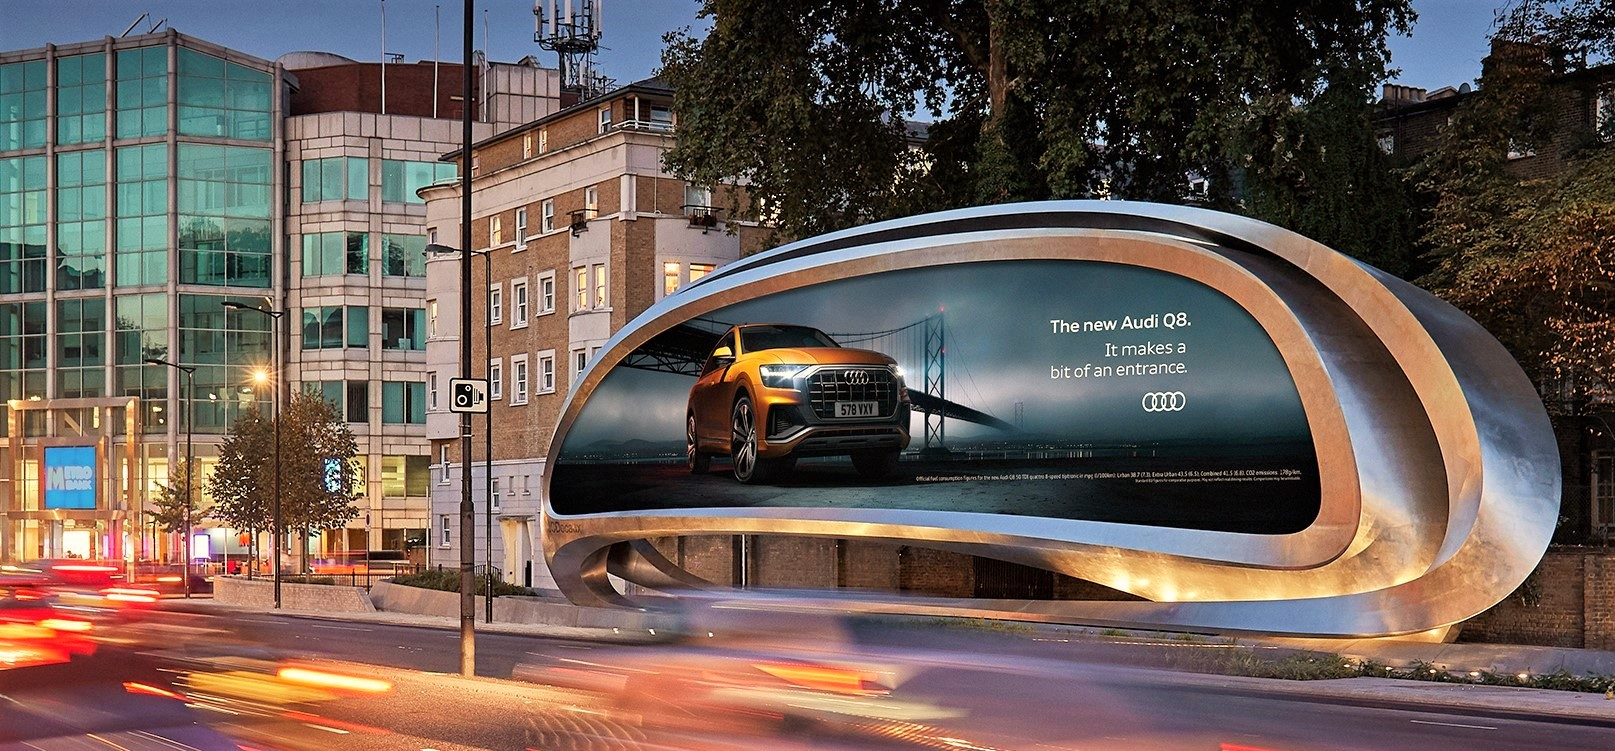
\includegraphics[width=0.9\paperwidth,height=0.45\paperheight]{resources/img/the_kensington_audi.jpg}
    };
\end{tikzpicture}

% Blue box (ugly way make it, but will do the job)
\begin{tikzpicture}[remember picture,overlay] 
    \node[anchor=north, yshift=-0.44\paperheight] at (current page.north){
        
\includegraphics[width=0.9\paperwidth,height=0.145\paperheight]{resources/img/blue_bg.jpg}

    };
    \node[anchor=north, yshift=-0.46\paperheight, xshift=-0.44\paperwidth, align=flush right, text width=0.7\paperwidth] 
    at (current page.north east) {
        \color{white} \Huge \textbf\documenttype\\
        \vspace{5mm}
        \color{white} \LARGE \documenttitle\\
    };
    \node[anchor=north, yshift=-0.64\paperheight, align=center, text width=0.7\paperwidth] at (current page.north) {
        \Large \textbf{Auteur:} Lucas GRELAUD\\
        \vspace{2mm}
        \Large \textbf{Période de mission :} 8 Février 2021 au 26 Août 2021
    };
    \node[anchor=north, yshift=-0.74\paperheight] at (current page.north) {
        \large
        \begin{tabular}{c@{\hskip 20mm}c@{\hskip 20mm}c}
    
            \textbf{\underline{Maître d'apprentissage}} & \textbf{\underline{Président du Jury}} & \textbf{\underline{Tuteur pédagogique}}\\
            \\
            \corpmanager & \jurypresident & \documentreviewer
        \end{tabular}
    };

\end{tikzpicture}

% ESIEA logo
\begin{tikzpicture}[remember picture,overlay] 
    \node[anchor=north, xshift=0.25\paperwidth] at (current page.north west){
        
\includegraphics[width=0.45\paperwidth,keepaspectratio]{resources/img/Logo_ESIEA_Baseline_blanc.png}
    };
\end{tikzpicture}

% Additionnal info
\begin{tikzpicture}[remember picture,overlay] 
    \node[anchor=south, yshift=-0.46\paperheight, xshift=-0.44\paperwidth, align=flush right, text width=0.7\paperwidth] 
    at (current page.south east) {
        \textbf\documenttype\\
        \vspace{5mm}
        \color{white} \LARGE \documenttitle\\
    };

\end{tikzpicture}

% JCDecaux logo
\begin{tikzpicture}[remember picture,overlay] 
    \node[anchor=south, yshift=15mm] at (current page.south){
        
\includegraphics[width=0.25\paperwidth,keepaspectratio]{resources/img/Logo_JCDecaux_seul_without_baseline.jpg}
    };
\end{tikzpicture}

\end{titlepage}



  %%%%%%%%%%%%%
  %% indexes %%
  %%%%%%%%%%%%%

  % disclosure statement - uncomment if needed
  % %!TEX root = ../main.tex

\addchap{Blocking notice}

This thesis may not be made accessible to third parties, with the exception of the supervising lecturers and authorized members of the administration, without the express consent of the company and the author.
In justified cases of suspicion, the thesis or parts thereof may be subjected by the FHDW to a plagiarism check by a plagiarism software provider and temporarily stored on FHDW-specific databases set up there.
The blocking notice is not effective in the event of a plagiarism check.
Reproduction and publication of the thesis without express permission - even in excerpts - is not permitted.

  % \newpage

  % executive summary - uncomment if needed
  %!TEX root = ../main.tex
\chapter*{Executive Summary}
It is farley known that the subject of computer security is a known issue the development of application by industries.
This issue is manly due to the fact that most of the development are side product of industries used to fulfil a 
technical need.
\newline This problematic is all the more significant when industries try to optimize their information system 
infrastructure by using containerized technologies and Cloud Computing at the same time.

In this thesis, we will try to find solutions and means to solve this ever-growing issue of securing the development and
deployment pipeline o containerized application. Then, after a careful selection, we will implement some of these solutions
on different parts of the pipeline and evaluate them.
\newline This work will also demonstrate the need of cooperation between security, architecture, infrastructure and 
development teams to achieve this goal.

The conclusion will follow with a first return of experience  of the implemented solution and associated results.
This par will include booth parts of  problematic.

Finally, we will discuss the future of the project and the possible tasks the company may need to accomplish to fulfil
its goal, more specifically on the training aspect.
  \newpage
  %!TEX root = ../main.tex
\chapter*{Résumé Analytique}
aaaaaaaaaaaaaaaaaaaaaaaaaaaaaaaaa
  \newpage

  % acknowledgment -  uncomment if needed
  % //TODO: Retirer // pour activer les remerciements
  %% //TODO : Remplir la page de remerciement

\chapter*{Remerciements}
Ce mémoire de mission de fin d'études constitue l'épilogue de trois riches et chaleureuses années d'apprentissage au sein de l'équipe de
sécurité du Groupe JCDecaux. C'est donc pourquoi je souhaiterais remercier 
  %\newpage

  % table of contents
  \tableofcontents
  \newpage

  %%%%%%%%%%%%%
  %% content %%
  %%%%%%%%%%%%%
  
  % insert chapter files here like this:
  %!TEX root = ../main.tex
\chapter{Introduction}

Cette mission de fin d'étude clôture trois années d'apprentissage réalisées au sein de l'équipe de sécurité informatique 
du Groupe JCDecaux. Elle permet aussi de finaliser un travail de longue haleine visant à sécuriser et moderniser
la chaîne de production des applications et outils exploités par le groupe et ses filiales.

\section{Le Groupe JCDecaux}
JCDecaux est un groupe industriel international fondée en France en 1964 par Jean-Claude Decaux et spécialisé dans 
l'affichage publicitaire urbain. Principalement connue pour son mobilier urbain (Abribus, MUPI\footnote{Mobilier Urbain 
Pour l'Information - Panneau d'affichage de 2m² dont l'une des faces est réservée pour les collectivités.}, Senior\footnote{
Panneau d'affichage de 4m² en fixation murale ou aérienne.}), l'entreprise familiale a su se hisser en tant que leader de 
la communication extérieure et est reconnue comme étant N°1 mondiale dans ce domaine depuis 2001. Le Chiffre d'Affaires du 
groupe était de 3 890.2 M€ en 2019.

La notoriété du Groupe JCDecaux s'explique par sa présence dans plus de 80 pays répartis sur tous les continents, mais
aussi et surtout par la qualité des services proposés tant auprès des collectivités locales qu'aux annonceurs.
Cette recherche de qualité, d'esthétique et d'innovation dans le mobiliers urbains fait partie intégrante des valeurs de 
l'entreprise et représente une réelle fierté pour ses 12 300 collaborateurs. 

\section{L'équipe Sécurité des Systèmes d'Informations}
\begin{wrapfigure}{R}{0.27\textwidth} 
    \centering 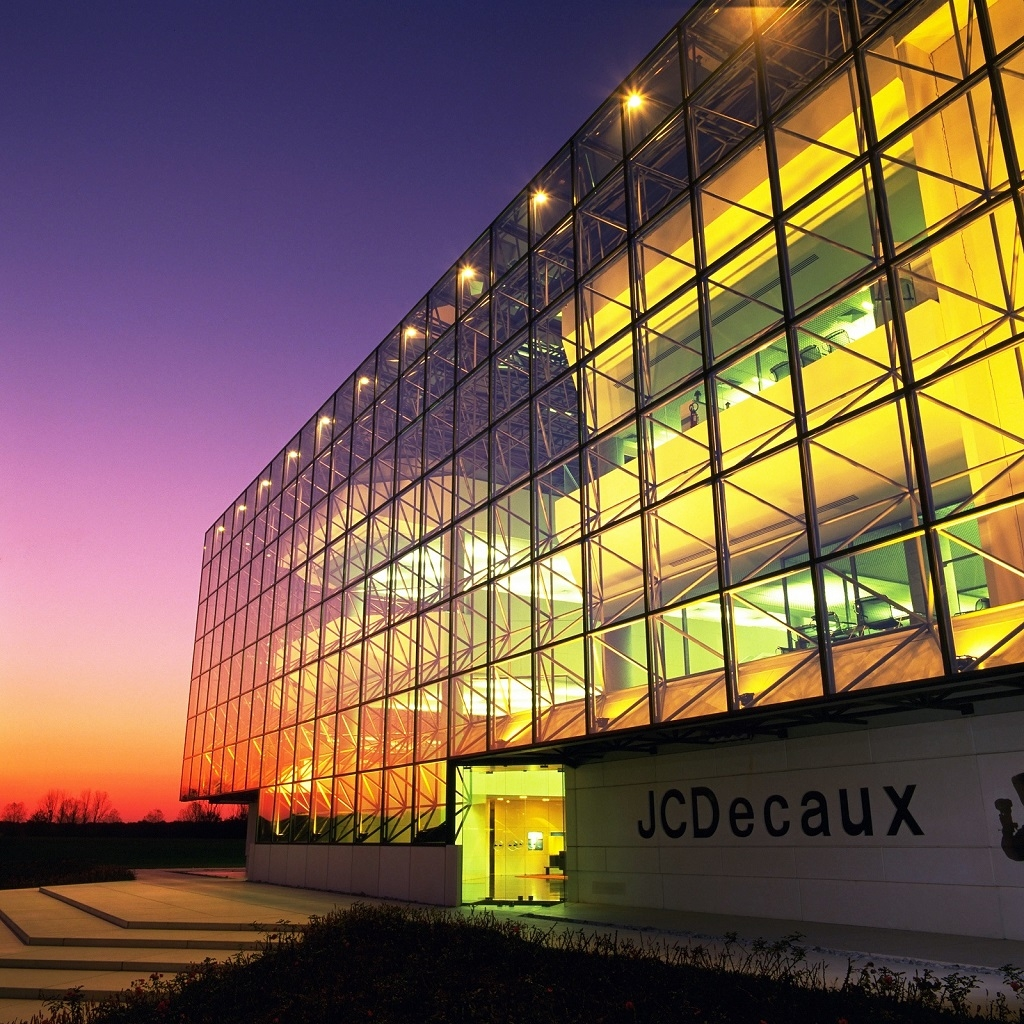
\includegraphics[width=0.25\textwidth]{resources/img/jcd_pla_front.jpg}
    \centering Siège de Sainte Apolline
\end{wrapfigure}
En 2013, la \ac{DSI} Groupe s'est pourvu d'une équipe dédiée à la \ac{SSI}.
Cette décision faisait suite à l'augmentation progressive des déploiements de systèmes de diffusion publicitaires numériques et
de la montée en puissance de la diffusion programmatique.

L'équipe \ac{SSI} Groupe de JCDecaux est localisée sur le plateau de la \ac{DSI}, au siège de Sainte-Apolline, Plaisir.
Elle est actuellement composée de trois personnels internes (le \ac{RSSI}, un ingénieur \ac{SSI}, un apprenti) et est complémenté 
par trois personnels externes en prestation.
\newpage
Les missions de cette équipe portent tant sur l'aspect organisationnel (Analyse de risque, gestion des politiques, sensibilisation),
l' opérationnel (SOC, conformité, veille phishing) que sur la qualification technique des systèmes et infrastructures. L'équipe propose
ainsi ces services au Groupe et à ses Filiales afin de sécuriser leurs systèmes.

\section{Publicité et développement applicatif}
De par la complexité et la volatilité du secteur publicitaire (publicité programmatique, booking de campagne, diffusion numérique), 
le Groupe JCDecaux se doit de disposer d'applications adaptées aux différents métiers de la publicité. 
Pour la réalisation de ces applications, le Groupe dispose d'équipes de développement interne dans une majorité des \ac{BU} 
de ses DSI (Groupe \& Filiales).

Depuis 2016, ces équipes de développement  ont mis en place dans leur projet des méthodes agiles; afin 
d'accélérer leurs temps de développement ainsi qu'améliorer la fiabilité et flexibilité de leurs applications.
Ce changement de doctrine sur les méthodes de gestion de projet a permis une réduction de la complexité des applications produites
grâce notamment à leur modularisation et favorise leurs réemplois pour tout ou partie dans les filiales du Groupe JCDecaux.

\section{Automatisation et conteneurisation du Si}
Conséquence de l'augmentation du nombre de composant applicatif dans le SI, le nombre de serveurs et machines virtuelles exploités par 
la \ac{DSI} n'a cessé de croître durant les cinq dernières années.

Pour palier à la complexité de gestion induite par cette augmentation, la \ac{DSI} Groupe s'est pourvu en outils et méthodes pour 
automatiser les tâches les plus courantes tel que l'initialisation des serveurs, le patch management ou encore le déploiement des
applications. Cet outillage a commencé par le développement et la mise en production d'une \ac{CMP} reliée à notre \ac{CMDB}, réel atout 
pour les équipes opérationnelles, puis la mise en place de script Ansible\footnote{Ansible est une plate-forme \ac{FOSS} développée par
RedHat servant à la gestion de déploiement applicatif au travers d'une simple connexion \ac{SSH}}

Depuis 2018, la \ac{DSI} Groupe et la \ac{DSI} France coopèrent dans un programme de déploiement des applications métier sous la forme
de conteneurs sur une infrastructure Kubernetes managé sur \ac{AWS}, le Cloud Provider de JCDecaux. Il vise à la simplification
déploiement applicatif en fournissant une couche d'abstraction unique et standard pour l'ensemble des équipes de développement du Groupe.

Ce programme est en phase de généralisation au sein du Groupe JCDecaux, mais un certain nombre de points relatif à la sécurisation des
applications, conteneurs et cluster Kubernetes sont à résoudre avant de pouvoir mettre cette technologie à disposition des filiales.

\section{Problématiques de sécurité}
Comme pour toute infrastructure hébergée par ou pour le Groupe JCDecaux, cette plateforme Kubernetes se doit de respecter un ensemble de 
règles et de principes définies par les IT Security Policies\footnote{FR: Politiques de sécurité Informatique}. Ces documents, 
regroupés par domaines (Réseau, Identité, Vulnérabilité, Données, etc..), régissent en effet l'aspect "Sécurité informatique" de tout projet
réalisés par les équipes du Groupe et les guides dans leurs développements.

Afin d'attester du niveau de conformité et de sécurité de la nouvelle plateforme, l'équipe \ac{SSI} à fait exécuter en externe un audit 
technique de cette dernière. Réalisé en Juillet 2020 par XMCO, cet audit avait pour objectif d'étudier le niveau de sécurité courant de 
l'environnement \ac{EKS} de JCDecaux (découverte et tentative d'exploitation de Vulnérabilités); ainsi que de fournir un certain nombre 
de recommandations visant à assurer la sécurité de la plateforme suite à sa généralisation.

Cet audit a permis de mettre en évidence de nombreuses de faiblesses et / ou défaut de conception de la plateforme Kubernetes. 
Suite à la restitution et analyse du compte-d'audit, plusieurs chantiers ont ainsi émergés :
\begin{enumerate}
    \item Cloisonnement de l'infrastructure
    \begin{itemize}
        \item Ségmentation des clusters en fonction des \ac{BU}
        \item Durcissement des règles réseau
    \end{itemize}
    \item Contrôle des déploiements
        \begin{itemize}
        \item Intégration de protection contre objets dangereux
        \item Application des PodSecurityPolicy
        \item Ajout de règles OpenPolicyAgent aux contrôleurs d'admission
    \end{itemize}
    \item Contrôle d'accès et secrets
    \begin{itemize}
        \item Renforcement du composant kube2iam
        \item Sécurisation du bastion SSH et des serveurs de rebonds
        \item Gestion et rotation des secrets
    \end{itemize}
    \item Sensibilisation et validation
    \begin{itemize}
        \item Mise en place de guides pour les développement / déploiement
        \item Sensibilisation des équipes
        \item Standardisation des déploiements
        \item Validation des images et des applications
    \end{itemize}
\end{enumerate}

\pagebreak

\section{La mission et ces objectifs}

Comme énoncé précédemment, quatre chantiers de remédiation sont à réaliser afin de rendre la plateforme Kubernetes conforme aux politiques
de sécurité informatique du groupe.

Le chantier de cloisonnement de l'infrastructure Kubernetes ainsi que celui relatif au contrôle d'accès sont en cours de 
finalisation. Ils ont en effet été lancés directement à la suite de l'audit.
\linebreak Le chantier de contrôle des déploiements est partiellement réalisé et celui de la sensibilisation reste à démarrer. C'est donc 
de à ces deux derniers que nous allons nous intéresser.

Les objectifs de ma mission de fin d'études sont exprimés de la façon suivante :
\begin{enumerate}
    \item Objectifs organisationnels : 
    \begin{itemize}
        \item Revue des procédures de qualification sécurité des applications, conteneurs et de déploiements
        \item Revue des procédures de gestion opérationnel de la sécurité des clusters Kubernetes
        \item Production de ressources visant à la standardisation des déploiements sur les clusters
        \item Production de guides et ressources visant à la sécurisation des développements pour Kubernetes
    \end{itemize}
    \item Objectifs techniques:
    \begin{itemize}
        \item Analyse des moyens techniques existants au sein du groupe et évaluation de leur efficacité.
        \item Consolidation et optimisation des moyens techniques existants.
        \item Qualification de nouvelles solutions techniques visant l’amélioration de la sécurité de l’infrastructure Kubernetes du  groupe, 
        tant sur les phases développements que sur les phases de déploiement.
        \item Intégration des solutions retenues à l’infrastructure. 
    \end{itemize}
\end{enumerate}

Ma mission est donc en réalité constituée de deux phases, chacune mêlant des objectifs organisationnel et techniques:
\begin{itemize}
    \item Première phase : revoir et normaliser notre méthodologie de gestion de la sécurité des développements (applicatif et conteneur)
    \item Second temps : fournir des éléments techniques et opérationnels visant à maintenir un bon niveau de sécurité dans l'exploitation 
    de la plateforme Kubernetes. 
\end{itemize}


  \newpage

  % when using pandoc workflow instead, uncomment the following
  % \input{chapter/out.tex}
  % \newpage

  %%%%%%%%%%%%%
  %% closing %%
  %%%%%%%%%%%%%
  
  % acronyms
  %!TEX root = ../main.tex

\addchap{Liste des acronymes}

\begin{acronym}[ABCD]
	% declare your own acronyms here:
	\acro{RSSI}{Responsable de la Sécurité des Systèmes d'Information}
	\acro{SSI}{Sécurité des Systèmes d'Information}
	\acro{DSI}{Direction des Systèmes d'Information}
	\acro{SOC}{Security Operation Center}
	\acro{AWS}{Amazon Web Services}
	\acro{BU}{Business Unit}
	\acro{CMP}{Cloud management Platform}
	\acro{CMDB}{Configuration Management DataBase}
	\acro{K8S}{Kubernetes}
	\acro{SI}{Système d'Information}
	\acro{SDLC}{Software Development Life Cycle}
	\acro{SAMM}{Software Assurance Maturity Model}
	\acro{RBAC}{Role-Base Access Control}
	\acro{KPI}{Key Performance Indicator}
	\acro{NIST}{National Institute of Standards and Technology}
	\acro{SAFECODE}{Software Assurance Forum for Excellence in Code}
	\acro{IAM}{Identity and Access Management}
	\acro{VCS}{Version Control Sytem}
	\acro{CI}{Continuous Integration}
	\acro{CD}{Continuous Delivery}
	\acro{SAST}{Static Application Security Testing}
	\acro{DAST}{Dynamic Application Testing}
	\acro{IAST}{Interactive Application Security Testing}
	\acro{OWASP}{Open Web Application Security Project}
	\acro{BPMN}{Business Process Model and Notation}
	\acro{DAF}{Directeur Administratif et Financer}
	\acro{npr}{non-production}
	\acro{ECR}{Elastic Cloud Registry}
	\acro{ACL}{Access Control List}
\end{acronym}
  \newpage

  % list of figures
  %\listoffigures
  %\newpage

  % list of tables
  %\listoftables
  %\newpage

  % list of listings
  %\listoflistings
  %\newpage
  % list of references
  %!TEX root = ../main.tex

\addchap{Références}

\defbibheading{book}{\section*{Monographien}}
\defbibheading{article}{\section*{Beiträge in Zeitungen und Zeitschriften}}
\defbibheading{incollection}{\section*{Beiträge in Sammelbänden}}
\defbibfilter{incollection}{
    type=inproceedings or    
    type=incollection or
    type=inbook
}
\defbibheading{paper}{\section*{Papers}}
\defbibfilter{paper}{
    type=thesis or
    type=report
}
\defbibheading{online}{\section*{Internetquellen}}
\defbibheading{jurisdiction}{\section*{Rechtsprechung}}
\defbibheading{company}{\section*{Unternehmensunterlagen}}
\defbibheading{uncited}{\section*{Unzitierte Quellen}}
\defbibcheck{uncited}{
  \ifciteseen
    {\skipentry}
    {}
}

\setlength\bibitemsep{1.5\itemsep}
\setlength{\bibhang}{2em}

\begingroup
\sloppy

\printbibliography[heading=book,type=book]
\printbibliography[heading=article,type=article]
\printbibliography[heading=incollection,filter=incollection]
\printbibliography[heading=paper,filter=paper]
\printbibliography[heading=online,type=online]
\printbibliography[heading=jurisdiction,keyword=jurisdiction]
\printbibliography[heading=company,keyword=company]
%\printbibliography[heading=uncited,check=uncited]
%\nocite{*}

\endgroup

  \newpage

  % appendix - uncomment if needed
  % %!TEX root = ../main.tex

\addchap{Appendix}
\label{appendix}

% create a table of appendices here manually like this:
%  \contentsline{section}{\numberline{1}AppendixTitle}{\pageref{app:appendixlabel}}{app:appendixlabel}

\newpage

% input the appendix files here like this:
%  \input{appendix/appendix1.tex}
%  \newpage

  % \newpage

  % affirmation
  %%!TEX root = ../main.tex

\addchap{Declaration on honorg}

I hereby declare that I have prepared this thesis independently.
Only the sources and aids expressly named in the thesis have been used.
I have marked as such any ideas taken over verbatim or in spirit.
This work has not yet been submitted to any examination authority in the same or a similar form.
\vspace{20mm}

\location, \submissiondate
\vspace{10mm}

\underline{\hspace{8cm}}\\\documentauthor

\end{document}
